% Options for packages loaded elsewhere
\PassOptionsToPackage{unicode}{hyperref}
\PassOptionsToPackage{hyphens}{url}
%
\documentclass[
  12pt,
  a4paper,
]{article}
\usepackage{amsmath,amssymb}
\usepackage{setspace}
\usepackage{iftex}
\ifPDFTeX
  \usepackage[T1]{fontenc}
  \usepackage[utf8]{inputenc}
  \usepackage{textcomp} % provide euro and other symbols
\else % if luatex or xetex
  \usepackage{unicode-math} % this also loads fontspec
  \defaultfontfeatures{Scale=MatchLowercase}
  \defaultfontfeatures[\rmfamily]{Ligatures=TeX,Scale=1}
\fi
\usepackage{lmodern}
\ifPDFTeX\else
  % xetex/luatex font selection
\fi
% Use upquote if available, for straight quotes in verbatim environments
\IfFileExists{upquote.sty}{\usepackage{upquote}}{}
\IfFileExists{microtype.sty}{% use microtype if available
  \usepackage[]{microtype}
  \UseMicrotypeSet[protrusion]{basicmath} % disable protrusion for tt fonts
}{}
\makeatletter
\@ifundefined{KOMAClassName}{% if non-KOMA class
  \IfFileExists{parskip.sty}{%
    \usepackage{parskip}
  }{% else
    \setlength{\parindent}{0pt}
    \setlength{\parskip}{6pt plus 2pt minus 1pt}}
}{% if KOMA class
  \KOMAoptions{parskip=half}}
\makeatother
\usepackage{xcolor}
\usepackage[margin=1in]{geometry}
\usepackage{color}
\usepackage{fancyvrb}
\newcommand{\VerbBar}{|}
\newcommand{\VERB}{\Verb[commandchars=\\\{\}]}
\DefineVerbatimEnvironment{Highlighting}{Verbatim}{commandchars=\\\{\}}
% Add ',fontsize=\small' for more characters per line
\usepackage{framed}
\definecolor{shadecolor}{RGB}{248,248,248}
\newenvironment{Shaded}{\begin{snugshade}}{\end{snugshade}}
\newcommand{\AlertTok}[1]{\textcolor[rgb]{0.94,0.16,0.16}{#1}}
\newcommand{\AnnotationTok}[1]{\textcolor[rgb]{0.56,0.35,0.01}{\textbf{\textit{#1}}}}
\newcommand{\AttributeTok}[1]{\textcolor[rgb]{0.13,0.29,0.53}{#1}}
\newcommand{\BaseNTok}[1]{\textcolor[rgb]{0.00,0.00,0.81}{#1}}
\newcommand{\BuiltInTok}[1]{#1}
\newcommand{\CharTok}[1]{\textcolor[rgb]{0.31,0.60,0.02}{#1}}
\newcommand{\CommentTok}[1]{\textcolor[rgb]{0.56,0.35,0.01}{\textit{#1}}}
\newcommand{\CommentVarTok}[1]{\textcolor[rgb]{0.56,0.35,0.01}{\textbf{\textit{#1}}}}
\newcommand{\ConstantTok}[1]{\textcolor[rgb]{0.56,0.35,0.01}{#1}}
\newcommand{\ControlFlowTok}[1]{\textcolor[rgb]{0.13,0.29,0.53}{\textbf{#1}}}
\newcommand{\DataTypeTok}[1]{\textcolor[rgb]{0.13,0.29,0.53}{#1}}
\newcommand{\DecValTok}[1]{\textcolor[rgb]{0.00,0.00,0.81}{#1}}
\newcommand{\DocumentationTok}[1]{\textcolor[rgb]{0.56,0.35,0.01}{\textbf{\textit{#1}}}}
\newcommand{\ErrorTok}[1]{\textcolor[rgb]{0.64,0.00,0.00}{\textbf{#1}}}
\newcommand{\ExtensionTok}[1]{#1}
\newcommand{\FloatTok}[1]{\textcolor[rgb]{0.00,0.00,0.81}{#1}}
\newcommand{\FunctionTok}[1]{\textcolor[rgb]{0.13,0.29,0.53}{\textbf{#1}}}
\newcommand{\ImportTok}[1]{#1}
\newcommand{\InformationTok}[1]{\textcolor[rgb]{0.56,0.35,0.01}{\textbf{\textit{#1}}}}
\newcommand{\KeywordTok}[1]{\textcolor[rgb]{0.13,0.29,0.53}{\textbf{#1}}}
\newcommand{\NormalTok}[1]{#1}
\newcommand{\OperatorTok}[1]{\textcolor[rgb]{0.81,0.36,0.00}{\textbf{#1}}}
\newcommand{\OtherTok}[1]{\textcolor[rgb]{0.56,0.35,0.01}{#1}}
\newcommand{\PreprocessorTok}[1]{\textcolor[rgb]{0.56,0.35,0.01}{\textit{#1}}}
\newcommand{\RegionMarkerTok}[1]{#1}
\newcommand{\SpecialCharTok}[1]{\textcolor[rgb]{0.81,0.36,0.00}{\textbf{#1}}}
\newcommand{\SpecialStringTok}[1]{\textcolor[rgb]{0.31,0.60,0.02}{#1}}
\newcommand{\StringTok}[1]{\textcolor[rgb]{0.31,0.60,0.02}{#1}}
\newcommand{\VariableTok}[1]{\textcolor[rgb]{0.00,0.00,0.00}{#1}}
\newcommand{\VerbatimStringTok}[1]{\textcolor[rgb]{0.31,0.60,0.02}{#1}}
\newcommand{\WarningTok}[1]{\textcolor[rgb]{0.56,0.35,0.01}{\textbf{\textit{#1}}}}
\usepackage{longtable,booktabs,array}
\usepackage{calc} % for calculating minipage widths
% Correct order of tables after \paragraph or \subparagraph
\usepackage{etoolbox}
\makeatletter
\patchcmd\longtable{\par}{\if@noskipsec\mbox{}\fi\par}{}{}
\makeatother
% Allow footnotes in longtable head/foot
\IfFileExists{footnotehyper.sty}{\usepackage{footnotehyper}}{\usepackage{footnote}}
\makesavenoteenv{longtable}
\usepackage{graphicx}
\makeatletter
\def\maxwidth{\ifdim\Gin@nat@width>\linewidth\linewidth\else\Gin@nat@width\fi}
\def\maxheight{\ifdim\Gin@nat@height>\textheight\textheight\else\Gin@nat@height\fi}
\makeatother
% Scale images if necessary, so that they will not overflow the page
% margins by default, and it is still possible to overwrite the defaults
% using explicit options in \includegraphics[width, height, ...]{}
\setkeys{Gin}{width=\maxwidth,height=\maxheight,keepaspectratio}
% Set default figure placement to htbp
\makeatletter
\def\fps@figure{htbp}
\makeatother
\setlength{\emergencystretch}{3em} % prevent overfull lines
\providecommand{\tightlist}{%
  \setlength{\itemsep}{0pt}\setlength{\parskip}{0pt}}
\setcounter{secnumdepth}{5}
\newlength{\cslhangindent}
\setlength{\cslhangindent}{1.5em}
\newlength{\csllabelwidth}
\setlength{\csllabelwidth}{3em}
\newlength{\cslentryspacingunit} % times entry-spacing
\setlength{\cslentryspacingunit}{\parskip}
\newenvironment{CSLReferences}[2] % #1 hanging-ident, #2 entry spacing
 {% don't indent paragraphs
  \setlength{\parindent}{0pt}
  % turn on hanging indent if param 1 is 1
  \ifodd #1
  \let\oldpar\par
  \def\par{\hangindent=\cslhangindent\oldpar}
  \fi
  % set entry spacing
  \setlength{\parskip}{#2\cslentryspacingunit}
 }%
 {}
\usepackage{calc}
\newcommand{\CSLBlock}[1]{#1\hfill\break}
\newcommand{\CSLLeftMargin}[1]{\parbox[t]{\csllabelwidth}{#1}}
\newcommand{\CSLRightInline}[1]{\parbox[t]{\linewidth - \csllabelwidth}{#1}\break}
\newcommand{\CSLIndent}[1]{\hspace{\cslhangindent}#1}
\newcommand{\docTitle}{Non-Parametric Biosimilatiry Assessment for Small Sample Sizes}
\usepackage{pgfplots}
\usepackage{fvextra}
\DefineVerbatimEnvironment{Highlighting}{Verbatim}{breaklines,commandchars=\\\{\}}
\usepackage[skins]{tcolorbox}
\usepackage{listings}
\usepackage{booktabs}
\usepackage{setspace}
\usepackage{titling}
\pgfplotsset{compat=1.18}
\usepackage{tikz}
\usepackage{tikz-3dplot}
\usetikzlibrary{arrows}
\usepackage{xcolor}
\usepackage{etoolbox}
\usepackage{amsmath}
\usepackage{caption}
\usepackage{enumitem}
\usepackage{varwidth}
\usepackage{mathrsfs}
\usepackage[nochapter, tocentry, owncaptions, tablegrid]{vhistory}
\usepackage{tasks}
\usepackage{scrlayer-scrpage}
\numberwithin{equation}{section}
\usepackage{lastpage}
\captionsetup[figure]{font=small,labelfont=small}
\usepackage{amsthm}
\theoremstyle{plain}
\newtheorem{theorem}{Theorem}
\theoremstyle{definition}
\newtheorem{defn}{Definition}
\newtheorem{xmpl}{Example}
\theoremstyle{remark}
\newtheorem{remark}{Remark}
\newtheorem{algorithm}{Algorithm} 
\newtheoremstyle{note}    % style name
{2ex}                     % above space
{2ex}                     % below space
{}                        % body font
{}                        % indent amount
{\scshape}                % head font
{.}                       % post head punctuation
{\newline}                % post head punctuation
{}                        % head spec
\theoremstyle{note}
\newtheorem{scnote}{Note}  

\pretitle{%
\begin{flushleft} \LARGE
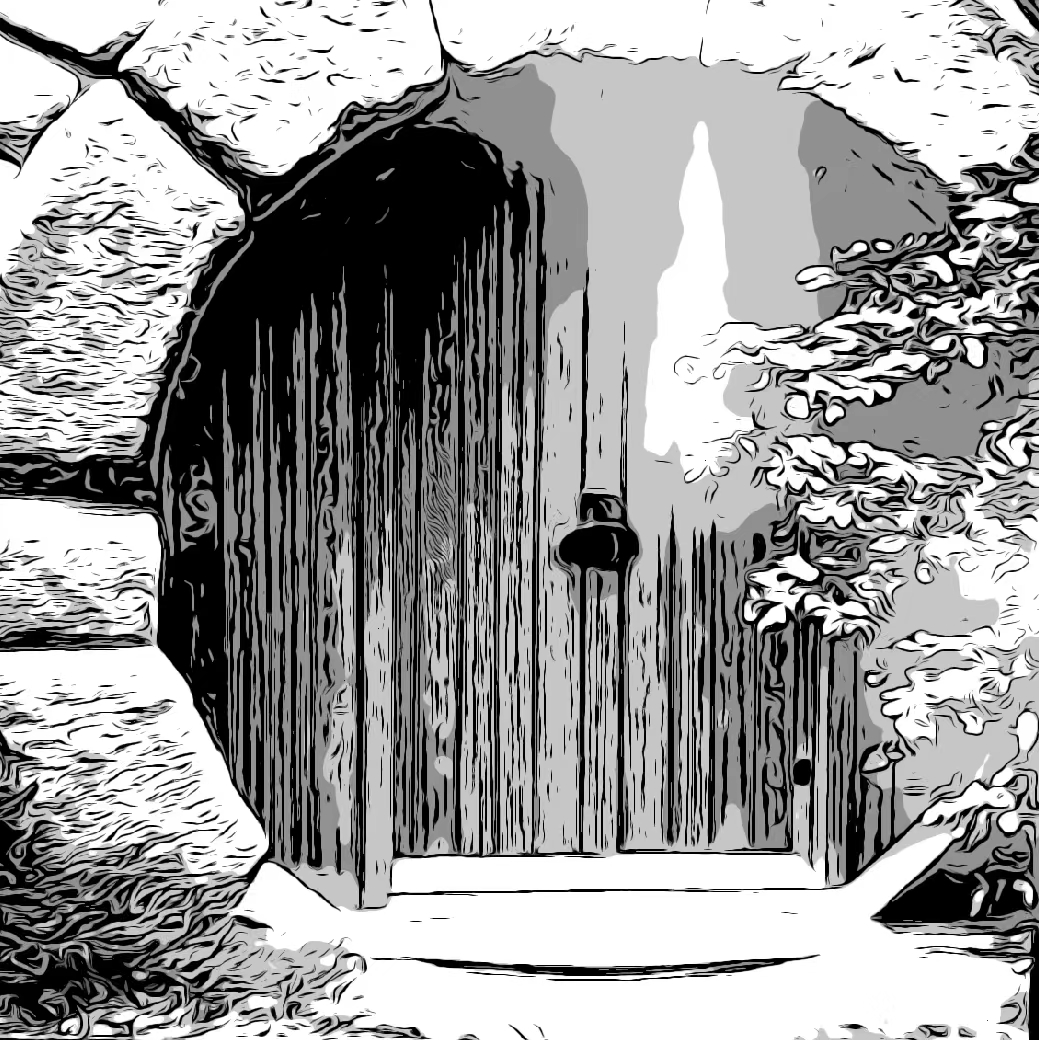
\includegraphics[width=2cm,height=2cm]{IH2.jpg}
\end{flushleft}
\begin{flushright} \LARGE
}

\posttitle{\end{flushright}}
\preauthor{\begin{flushright}}
\postauthor{\end{flushright}}
\predate{\begin{flushright}}
\postdate{\end{flushright}}

\ohead[]{Insight Hatch: Technical White Paper}
\ifoot{\hsize=350pt \docTitle\ -- Version \vhCurrentVersion}
\ofoot{\thepage~/~\pageref{LastPage}}
\cfoot[]{}


\ifLuaTeX
  \usepackage{selnolig}  % disable illegal ligatures
\fi
\IfFileExists{bookmark.sty}{\usepackage{bookmark}}{\usepackage{hyperref}}
\IfFileExists{xurl.sty}{\usepackage{xurl}}{} % add URL line breaks if available
\urlstyle{same}
\hypersetup{
  pdftitle={Non-Parametric IND Biosimilarity Assessment for Small Analytical Sample Sizes},
  pdfauthor={D Palahnuk},
  hidelinks,
  pdfcreator={LaTeX via pandoc}}

\title{Non-Parametric IND Biosimilarity Assessment for Small Analytical
Sample Sizes}
\usepackage{etoolbox}
\makeatletter
\providecommand{\subtitle}[1]{% add subtitle to \maketitle
  \apptocmd{\@title}{\par {\large #1 \par}}{}{}
}
\makeatother
\subtitle{\textit{BioSim 1}}
\author{D Palahnuk}
\date{\vhCurrentDate\\
version \vhCurrentVersion\\
\strut \\
InsightHatch: ``Non-Parametric Biosimilarity Assessment for Small
Analytical Sample Sizes when dealing with IND Dossier Data''\\
\textbf{IH-NonParBioSim-v}\textbf{\vhCurrentVersion}}

\begin{document}
\maketitle

{
\setcounter{tocdepth}{2}
\tableofcontents
}
\setstretch{1.25}
\hfill\break

\begin{versionhistory}
  \vhEntry{0.0}{2023.11.15}{DP}{Created!}
  \vhEntry{0.1}{2023.11.29}{DP}{Update with more graphics, andded R-code blocks and calculation framework}
  \vhEntry{0.2}{2023.12.03}{DP}{With the feedback of Wang Chen expanded and clarified for YZY discussions planned on 2023-12-05}
  \vhEntry{0.3}{2023.12.04}{DP}{Clarified the role of pdf for $x$ and $y$ inline with linear model effect on clinical outcome}
  \vhEntry{0.4}{2023.12.05}{DP}{Finalized draft for release to client}
\end{versionhistory}

\newpage

\setcounter{table}{0}

\hypertarget{bioequivalance-assessment-for-larger-n-with-assumed-underlying-normality}{%
\section{\texorpdfstring{BioEquivalance assessment for larger \(n\) with
assumed underlying
normality}{BioEquivalance assessment for larger n with assumed underlying normality}}\label{bioequivalance-assessment-for-larger-n-with-assumed-underlying-normality}}

We enter this discussion by following a well know reference
{[}\protect\hyperlink{ref-endrenyi_biosimilar_2017}{1}: Endrenyi L, et
al 2017{]} where the idea of using two different types of criteria for
analytical similarity based on absolute difference or relative
difference of a \emph{new test material} against an \emph{orginator
reference material} is statistically formulated. In the spirit of
keeping the derivation more compact we will only focus on the absolute
difference approach. The more curious reader may consult the reference
directly.

Basically, under the Fundamental Bio-equivalence Assumption, the ``In
Vitro-In Vivo Correlation'' (IVIVC) is to use the dissolution test as a
surrogate for human studies (i.e., when the drug absorption profiles in
terms of ``Area Under the Curve'' (AUC) or \(C_{\max }\) are similar, it
is assumed that they are therapeutically equivalent). In addition, one
of IVIVC's main roles is to assist in the quality control of functional
and/or structural characteristics during the manufacturing process.

For simplicity and illustration purposes, we will consider the case
where the relationship between CQA and clinical outcome is linear. The
nonlinear case can be similarly treated, albeit perhaps more
mathematically complicated.

Let \(x\) and \(y\) be the response of a ``Critical Quality Attribute''
CQA and the clinical outcome, respectively. In practice, if the CQA is
relevant to clinical outcome, it is assumed that the clinical outcome
can be predicted by the CQA accurately and reliably with some
statistical assurance. One of the statistical criteria is to examine the
degree of closeness (or the degree of relevance) between the observed
response \(y\) and the predicted response \(\hat{y}\) through an
established statistical model. \emph{It is worth noting here: We are
pursuing understanding the sensitivity of a clinical outcome as related
to the analytical variance of a CQA.}

To perform this examination, we will first study the association between
\(x\) and \(y\) and build up a model. Then, we will validate the model
based on some criteria. For simplicity, we assume that \(x\) (some
analytical quality measure) and \(y\) (some measurable clinically
dependent outcome) can be described by the following linear model: \[
y=\beta_0+\beta_1 x+\varepsilon
\] where \(\varepsilon\) follows a normal distribution with a mean of 0
and a variance of \(\sigma_e^2\). Suppose that \(n\) pairs of
observations \(\left(x_1, y_1\right), \ldots,\left(x_n, y_n\right)\) are
observed in a translation process. To define the notation, let \[
X^T=\left(\begin{array}{llll}
1 & 1 & \ldots & 1 \\
x_1 & x_2 & \ldots & x_n
\end{array}\right)
\] and \[
Y^T=\left(\begin{array}{llll}
y_1 & y_2 & \cdots & y_n
\end{array}\right) .
\]

Then, under model 3.1, the maximum likelihood estimates of the
parameters \(\beta_0\) and \(\beta_1\) are: \[
\left(\begin{array}{l}
\hat{\beta}_0 \\
\hat{\beta}_1
\end{array}\right)=\left(X^T X\right)^{-1} X^T Y
\] with \[
\operatorname{var}\left(\begin{array}{l}
\hat{\beta}_0 \\
\hat{\beta}_1
\end{array}\right)=\left(X^T X\right)^{-1} \sigma_e^2 .
\]

Furthermore, \(\sigma_e^2\) can be estimated by the mean squared error
(MSE), which is given by

\[
\hat{\sigma}_e^2=\frac{1}{n-2} \sum_{i=1}^n\left(y_i-\hat{y}_i\right)^2
\]

Thus, we have established the following relationship: \[
\hat{y}=\hat{\beta}_0+\hat{\beta}_1 x \text {. }
\]

For a given \(x=x_0\), suppose that the corresponding observed value is
given by \(y\); however, using Equation 3.2, the corresponding fitted
value is \(\hat{y}=\hat{\beta}_0+\hat{\beta}_1 x_0\). Note that
\(E(\hat{y})=\beta_0+\beta_1 x_0=\mu_0\) and \[
\operatorname{var}(\hat{y})=\left(\begin{array}{ll}
1 & x_0
\end{array}\right)\left(X^T X\right)^{-1}\left(\begin{array}{c}
1 \\
x_0
\end{array}\right) \sigma_e^2=c \sigma_e^2,
\] where \[
c=\left(\begin{array}{ll}
1 & x_0
\end{array}\right)\left(X^T X\right)^{-1}\left(\begin{array}{l}
1 \\
x_0
\end{array}\right) .
\]

Furthermore, \(\hat{y}\) is normally distributed with mean \(\mu_0\) and
variance \(c \sigma_e^2\), that is, \[
\hat{y} \sim N\left(\mu_0, c \sigma_e^2\right) .
\]

We may validate the translation model by considering how close an
observed \(y\) is to its predicted value \(\hat{y}\), which is fitted to
the regression model 3.2. To assess the closeness, we propose the
following two measures, which are based either on the absolute
difference or the relative difference between \(y\) and \(\hat{y}\):

Criterion I. \(\quad p_1=P\{|y-\hat{y}|<\delta\}\)\\

Criterion II.
\(\quad p_2=P\left\{\left|\frac{y-\hat{y}}{y}\right|<\delta\right\}\)\\

In this paper we only focus on Criterion I, in order to keep the overall
analysis shorter.

In other words, it is desirable to have a high probability that the
difference or the relative difference between \(y\) and \(\hat{y}\),
given by \(p_1\) and \(p_2\), respectively, is less than a clinically or
scientifically meaningful difference \(\delta\). Then, for either
\(i=1\) or 2 , it is of interest to test the following hypotheses: \[
H_0: p_i \leq p_0 \text { versus } H_a: p_i>p_0,
\] where \(p_0\) is some prespecified constant. The idea is to reject
\(H_0\) in favor of \(H_a\). In other words, we would like to reject the
null hypothesis \(H_0\) and conclude \(H_a\), which implies that the
established model is considered validated.

\hypertarget{considerations-of-what-this-is-really-all-about---and-why-we-are-pursuing-the-anlysis-this-way}{%
\subsubsection{Considerations of what this is really all about - and why
we are pursuing the anlysis this
way}\label{considerations-of-what-this-is-really-all-about---and-why-we-are-pursuing-the-anlysis-this-way}}

It makes sense to talk about what this above model formulation is really
representing. Firstly, we are trying to build a relationship of the
clinical outcome as it has some dependence on the product CQAs. And from
that position talk about the allowable or acceptable variance of the
CQAs with respect to this potential clinical impact. The underlying
imprtance of this assumes the follwing key elemtns in the model
construction:

\begin{enumerate}
\def\labelenumi{\arabic{enumi}.}
\tightlist
\item
  The relationship of the clinical outcome and CQA to some extent can be
  modeled or assessed.
\item
  We assume this relationship for \(y\) to \(x\), for the purposes of
  analysis, may be subject to MVLR (Multi-Variate Linear Regression).
\item
  There is enough data (i.e.~\(n\)) to assess for normality of the
  variances of the clinical outcome, and also perhaps the CQA measure of
  interest.
\item
  The aim is to build a statistical argument that the dependence of
  \(y\) can be tied to a definable `t-test' on \(x\) of sorts to assess
  CQA differnces and the potential impact on \(y\) the clinical outcome.
  With the formulation of the dependence of the prediction of the
  clinical outcome observation \(\hat{y}\)we have an insightful implied
  coupling to the variance of the CQA \(x\).
\end{enumerate}

\[
  x \sim N\left(\mu_{x}, c^* \sigma_x^2\right)\implies \hat{y} \sim N\left(\mu_0, c \sigma_e^2\right)
\] The implication here is that the underlying variance of the CQA is
closely related to the variance of the clinical outcome. Of note here is
the use of \(c^*\) vs \(c\) with the former being a z-score factor for
the CQAs and not the clinical outcome,

\hypertarget{measure-of-closeness-based-on-the-absolute-difference}{%
\subsection{Measure of Closeness Based on the Absolute
Difference}\label{measure-of-closeness-based-on-the-absolute-difference}}

It should be noted that we have \[
(y-\hat{y}) \sim N\left(0,(1+c) \sigma_e^2\right) \text {. }
\]

Therefore, \(p_1\) can be estimated by \[
\hat{p}_1=\Phi\left(\frac{\delta}{\sqrt{(1+c) \hat{\sigma}_e^2}}\right)-\Phi\left(\frac{-\delta}{\sqrt{(1+c) \hat{\sigma}_e^2}}\right)
\]

\hypertarget{understanding-this-formulation-for-p_1}{%
\subsubsection{\texorpdfstring{Understanding this formulation for
\(p_1\)}{Understanding this formulation for p\_1}}\label{understanding-this-formulation-for-p_1}}

\begin{itemize}
\tightlist
\item
  \(\Phi\) represents the cumulative distribution function (CDF) of the
  standard normal distribution.
\item
  \(\delta\) is a clinically or scientifically meaningful difference.
\item
  \(c\) and \(\hat{\sigma}_e^2\) are parameters related to the variance
  in the model.
\item
  The formula essentially calculates the probability that the absolute
  difference between the observed and predicted values is less than
  \(\delta\), under the assumption that the difference follows a normal
  distribution.
\end{itemize}

This formula likely comes from the properties of the normal distribution
and the specific context of the study, where \(\delta\) is a threshold
for deciding if a difference is significant, and \(\hat{\sigma}_e^2\) is
an estimate of the variance of errors in the model. The use of the CDF
\(\Phi\) twice with \(\delta\) and \(-\delta\) accounts for the absolute
difference being less than \(\delta\) in both positive and negative
directions.

To understand the derivation of the term \[
\frac{\delta}{\sqrt{(1+c) \hat{\sigma}_e^2}}
\] inside the cumulative distribution function (CDF) \(\Phi\) in the
equation \[
\hat{p}_1=\Phi\left(\frac{\delta}{\sqrt{(1+c) \hat{\sigma}_e^2}}\right)-\Phi\left(\frac{-\delta}{\sqrt{(1+c) \hat{\sigma}_e^2}}\right),
\] we need to consider the context of statistical hypothesis testing and
the normal distribution.

\begin{enumerate}
\def\labelenumi{\arabic{enumi}.}
\tightlist
\item
  Context of the Problem:
\end{enumerate}

\begin{itemize}
\tightlist
\item
  The term \(\delta\) represents a predetermined margin of difference,
  which is considered clinically or scientifically significant.
\item
  \(\hat{\sigma}_e^2\) is an estimate of the variance of the error term
  in the model.
\item
  The constant \(c\) is a scaling factor of variance in the statistical
  model.
\end{itemize}

\begin{enumerate}
\def\labelenumi{\arabic{enumi}.}
\setcounter{enumi}{1}
\tightlist
\item
  Normalization in the Standard Normal Distribution:
\end{enumerate}

\begin{itemize}
\tightlist
\item
  In a standard normal distribution, the variable of interest (say,
  \(y\)) is normalized by subtracting the mean and dividing by the
  standard deviation. This transforms the variable to have a mean of 0
  and a standard deviation of 1 .
\item
  In this context, \(\delta\) is akin to the difference from the mean.
  The expression \(\sqrt{(1+c) \hat{\sigma}_e^2}\) is the standard
  deviation of the distribution under consideration.
\end{itemize}

\begin{enumerate}
\def\labelenumi{\arabic{enumi}.}
\setcounter{enumi}{2}
\tightlist
\item
  Deriving the Expression:
\end{enumerate}

\begin{itemize}
\tightlist
\item
  The formula is normalizing the difference \(\delta\) with respect to
  the modified standard deviation \(\sqrt{(1+c) \hat{\sigma}_e^2}\).
  This is consistent with transforming a normal variable to a standard
  normal variable.
\item
  Specifically, if the differences in the model are assumed to follow a
  normal distribution with a certain variance, then \(\delta\) (the
  threshold of difference) is normalized by this standard deviation to
  understand its significance relative to the variability in the data.
\end{itemize}

\begin{enumerate}
\def\labelenumi{\arabic{enumi}.}
\setcounter{enumi}{3}
\tightlist
\item
  Conceptual Understanding:
\end{enumerate}

\begin{itemize}
\tightlist
\item
  This expression is essentially a Z-score, which is a common
  statistical measure used to describe a data point's relationship to
  the mean of a group of data points, in terms of standard deviations.
\item
  In the context of hypothesis testing, this normalized value is then
  used with the CDF \(\Phi\) to calculate the probability of observing a
  difference as extreme as \(\delta\), considering the variance in the
  data.
\end{itemize}

This transformation into a standard normal form allows the use of
standard normal distribution tables (or the CDF) to determine
probabilities, which is a common approach in statistical hypothesis
testing.

\hypertarget{the-variance-of-p_1}{%
\subsection{\texorpdfstring{The Variance of
\(p_1\)}{The Variance of p\_1}}\label{the-variance-of-p_1}}

Using the delta method through a Taylor expansion, for a sufficiently
large sample size \(n\), \[
\operatorname{var}\left(\hat{p}_1\right) \approx\left(\phi\left(\frac{\delta}{\sqrt{(1+c) \sigma_e^2}}\right)-\phi\left(\frac{-\delta}{\sqrt{(1+c) \sigma_e^2}}\right)\right)^2 \frac{\delta}{2(1-\delta)(n-2) \sigma_e^2},
\] where \(\phi(z)\) is the probability density function of a standard
normal distribution. Furthermore,
\(\operatorname{var}\left(\hat{p}_1\right)\) can be estimated by
\(V_1\), where \(V_1\) is given by \[
V_1=\frac{2 \delta^2}{(1+c)(n-2) \hat{\sigma}_e^2} \phi^2\left(\frac{\delta}{\sqrt{(1+c) \hat{\sigma}_e^2}}\right) .
\]

\hypertarget{testing-the-null-hypothesis}{%
\subsection{Testing the null
hypothesis}\label{testing-the-null-hypothesis}}

By Slutsky's theorem, \(\hat{p}_1-p_0 / \sqrt{V_1}\) can be approximated
by a standard normal distribution. For the testing of the hypotheses
\(H_0: p_1 \leq p_0\) versus \(H_a: p_1>p_0\), we would reject the null
hypothesis \(H_0\) if \[
\frac{\hat{p}_1-p_0}{\sqrt{V_1}}>z_{1-\alpha}
\] where \(z_{1-\alpha}\) is the \(100(1-\alpha)\) th percentile of a
standard normal distribution

\hypertarget{implications-for-cqa-range-limitting}{%
\subsection{Implications for CQA range
limitting}\label{implications-for-cqa-range-limitting}}

This gives us a general recipe to approach these Biosimilarity
assessment problems.

To limit variation in clinical outcomes, we aim to set boundaries on the
range of CQAs. Based on our initial assumption of linearity: \[
\hat{y}=\hat{\beta}_0+\hat{\beta}_1 x .
\]

The differential form, where \(\beta_1\) is a regression constant,
becomes: \[
\partial \hat{y}=\beta_1 \partial x .
\]

This supports the general notion: \[
x \sim N\left(\mu_x, c^* \sigma_x^2\right) \Longrightarrow \hat{y} \sim N\left(\mu_0, c \sigma_e^2\right) .
\]

From here, one might hypothesize: \[
c^* \sim \beta_1 c .
\]

It is worth noting that in the absence of clinical assessment this
hypothesis may challenged by health authorities. However, to-date there
does not seem to be batter approach that has been put forward in the
literature.

This hypothesis provides a framework for approaching Biosimilarity
assessment problems:

\begin{enumerate}
\def\labelenumi{\arabic{enumi}.}
\tightlist
\item
  We must assume that we can preserve the linear mapping
  \(\hat{y}=\hat{\beta}_0+\hat{\beta}_1 x\).
\item
  Analyze the probability of variance in \(x\) and establish control
  limits to ensure minimal impact of CQA changes on the clinical outcome
  \(y\).
\item
  Leverage the relationship \(c^* \sim \beta_1 c\) as a general rule
\item
  Tune \(c^*\) in \(x \sim N\left(\mu_x, c^* \sigma_x^2\right)\) to
  maintain expected clinical outcomes
\item
  Apply a risk-based approach to adjust \(c^*\) based on the potential
  impact of a CQA.
\end{enumerate}

In cases where the probability distribution function (pdf) is non-normal
or unknown, it's reasonable to adopt a non-parametric method for
variance assessment of \(x\). This approach suggests that the linear
mapping could preserve the non-parametric (nonnormal pdf)
characteristics from \(x\) to \(y\).

The leap to non-parametric methods is perhaps significant. We emphasize
the conditions under which this transition is valid or more useful. For
Clinical IND phase 1 studies and comparison of data - there is little
room beyond this approach, unless there is access to additional data.
Note that the non-parametric approach is a contingency for when
normality assumptions do not hold, and when the number of samples is
also low.

\newpage

\hypertarget{bioequivalance-assessment-for-smaller-n-with-assumed-underlying-normality}{%
\section{\texorpdfstring{BioEquivalance assessment for smaller \(n\)
with assumed underlying
normality}{BioEquivalance assessment for smaller n with assumed underlying normality}}\label{bioequivalance-assessment-for-smaller-n-with-assumed-underlying-normality}}

\hypertarget{addressing-small-samples-sizes-of-n}{%
\subsection{\texorpdfstring{Addressing Small Samples Sizes of
\(n\)}{Addressing Small Samples Sizes of n}}\label{addressing-small-samples-sizes-of-n}}

In previous sections, we discussed scenarios involving larger sample
sizes, typically \(n>12\), where the Taylor expansion is applicable for
deriving estimates of the variance of \(p_i\). This method, however, may
not be suitable for smaller sample sizes.

For cases where the sample size is notably small, and the assumption of
normality is questionable, an alternate estimation strategy is required
for \(p_i\).

We propose examining two distinct approaches, particularly relevant for
small sample sizes:

\hypertarget{estimation-for-small-samples-utilizing-range-based-standard-deviation-under-assumed-normal-distribution}{%
\subsection{Estimation for Small Samples Utilizing Range-Based Standard
Deviation under Assumed Normal
Distribution}\label{estimation-for-small-samples-utilizing-range-based-standard-deviation-under-assumed-normal-distribution}}

In scenarios with small sample sizes, where it's reasonable to assume
that the measure's variance is normal or nearly normal, a range-based
estimate can be used to approximate the variable of interest's variance.

\begin{itemize}
\tightlist
\item
  A commonly used rule of thumb for estimating the sample standard
  deviation in small samples is:
\end{itemize}

\[
\sigma \approx \frac{\text { sample range }}{4}
\]

However, this method has limitations, particularly in its failure to
account for the sample size dependent uncertainty of standard deviation.

A noteworthy advancement was proposed by undergraduate math researchers
at Rose-Hulman in 2012
{[}\protect\hyperlink{ref-ramirez_improving_2012}{2}{]}. Their work,
based on R simulations, suggests an improved range-based estimate:

\[
\sigma \approx \frac{\text { range }}{3 \sqrt{\ln n}-1.5}
\]

agin considering the general notion: \[
x \sim N\left(\mu_x, c^* \left[\frac{\text { range }}{3 \sqrt{\ln n}-1.5} \right] ^2\right) \Longrightarrow \hat{y} \sim N\left(\mu_0, c \sigma_e^2\right) .
\]

This refined approach leverages the sample range as a surrogate for
variability, a typical method in small sample size analysis. It still,
however, hinges on the assumption of normal distribution for calculating
probabilities using the CDF \(\Phi\). This methodology can streamline
the TOST analysis z-score calculation, particularly when there is a
prior basis to assert that both the reference originator material and
new test articles exhibit normal variance. This situation might occur,
for example, with similar antibodies under comparable testing
conditions. However, in the majority of biosimilar Investigational New
Drug (IND) studies, there often exists limited understanding of the
original analytical method and process variance for a given Critical
Quality Attribute (CQA), making this approach less commonly applicable.

\newpage

\hypertarget{bioequivalance-assessment-for-smaller-n-with-no-assumed-underlying-normality}{%
\section{\texorpdfstring{BioEquivalance assessment for smaller \(n\)
with no assumed underlying
normality}{BioEquivalance assessment for smaller n with no assumed underlying normality}}\label{bioequivalance-assessment-for-smaller-n-with-no-assumed-underlying-normality}}

When we have a small sample size that we would like to evaluate,
assuming the sample pdf is not always known a priori. We consider here
the approach of using a non-parametric assessment of the originator data
(for some sample size \(n_{RP}\)) to our new test data (for some sample
size \(n_{test}\)).

\hypertarget{non-parametric-approach-for-small-samples}{%
\subsection{Non-Parametric Approach for Small
Samples}\label{non-parametric-approach-for-small-samples}}

Non-parametric methods don't assume a specific distribution for the
data, making them suitable for small samples where normality cannot be
assumed.

\begin{itemize}
\item
  \textbf{Boostrapping:} One approach could involve using bootstrapping
  or resampling techniques. By resampling the small dataset (with
  replacement) many times, we can create a distribution for
  \(\hat{p}_i\) for \(x\) estimates. This distribution can then be used
  to determine confidence intervals or test hypotheses without relying
  on normal distribution assumptions.
\item
  \textbf{Rank Based Statistics:} Another approach could be to use
  rank-based statistics. For example, one could calculate \(p_i\) for
  \(x\) based on the ranks of the observed values rather than their
  actual magnitudes. This could involve comparing the ranks of the
  observed values to the expected ranks under some null hypothesis.
\item
  \textbf{Applied ML:} A more creative approach might involve leveraging
  machine learning algorithms that are robust to small sample sizes and
  do not assume normality. For example, decision tree-based methods or
  certain types of Bayesian models might be able to provide insights
  into the distribution and behavior of \(p_i\) under small sample
  conditions.
\end{itemize}

The key challenge is to adapt the method to the limitations of small
sample sizes while still capturing the essence of what \(p_i\) for \(x\)
represents in the context of the study. These approaches offer ways to
estimate \(p_i\) for \(x\) that are less reliant on large sample theory
and normality assumptions. The specific choice depends on the nature of
the data and the exact requirements of the analysis.

\hypertarget{employing-rank-based-statstics}{%
\subsection{Employing Rank Based
Statstics}\label{employing-rank-based-statstics}}

A rank-based approach can be particularly useful in non-parametric
statistics, especially when dealing with small sample sizes or when the
normality assumption is questionable.

\hypertarget{basic-outline-or-recipe-for-using-rank-based-statistics-to-estimate-p_i}{%
\subsubsection{\texorpdfstring{Basic outline or ``recipe'' for using
rank-based statistics to estimate
\(p_i\):}{Basic outline or ``recipe'' for using rank-based statistics to estimate p\_i:}}\label{basic-outline-or-recipe-for-using-rank-based-statistics-to-estimate-p_i}}

\begin{enumerate}
\def\labelenumi{\arabic{enumi}.}
\tightlist
\item
  Understand the Context and Data:
\end{enumerate}

\begin{itemize}
\tightlist
\item
  Identify the variable of interest (e.g., difference between observed
  and predicted values, response times, etc.).
\item
  Gather your small sample data set.
\end{itemize}

\begin{enumerate}
\def\labelenumi{\arabic{enumi}.}
\setcounter{enumi}{1}
\tightlist
\item
  Rank the Data:
\end{enumerate}

\begin{itemize}
\tightlist
\item
  Assign ranks to each data point in your sample. The smallest value
  gets rank 1 , the next smallest rank 2, and so on.
\item
  In case of ties (equal values), assign the average of the ranks that
  would have been assigned to all the tied values.
\end{itemize}

\begin{enumerate}
\def\labelenumi{\arabic{enumi}.}
\setcounter{enumi}{2}
\tightlist
\item
  Calculate Rank Statistics:
\end{enumerate}

\begin{itemize}
\tightlist
\item
  Depending on your specific hypothesis or research question, calculate
  relevant rank-based statistics. Examples include:

  \begin{itemize}
  \tightlist
  \item
    \textbf{Wilcoxon Signed-Rank Test:} Used for comparing two related
    samples or repeated measurements (aka ``paired data'') on a single
    sample to assess whether their population mean ranks differ.
  \item
    \textbf{Mann-Whitney U Test:} Used to compare differences between
    two independent groups when the dependent variable is ordinal or
    continuous but not normally distributed. Applicable to ``two
    groups'', non-paired'', with ``unequal sample sizes''.
  \item
    \textbf{Kruskal-Wallis H Test:} An extension of the Mann-Whitney U
    Test for more than two groups. Applicable to ``two or more groups'',
    non-paired'', with ``unequal sample sizes''.
  \end{itemize}
\end{itemize}

\begin{enumerate}
\def\labelenumi{\arabic{enumi}.}
\setcounter{enumi}{3}
\tightlist
\item
  Estimate \(p_i\) for \(x\) Using Rank Statistics:
\end{enumerate}

\begin{itemize}
\tightlist
\item
  The specifics of this step depend on your hypothesis and data. For
  instance, if you're testing if the median of the differences is
  significantly different from zero, you might use the Wilcoxon
  Signed-Rank Test.
\item
  The test statistic from these rank-based tests can be used to
  calculate a \(p\)-value, which indicates the probability of observing
  the obtained result, or more extreme, under the null hypothesis.
\end{itemize}

\begin{enumerate}
\def\labelenumi{\arabic{enumi}.}
\setcounter{enumi}{4}
\tightlist
\item
  Interpret the Results:
\end{enumerate}

\begin{itemize}
\tightlist
\item
  A small \(p\)-value (typically \textless{} 0.05, 95\% confidence
  interval) suggests that the observed effect (e.g., difference between
  groups) is statistically significant and not likely due to chance.
\item
  Interpret the results in the context of your research question, taking
  into account the limitations of rank-based methods.
\end{itemize}

\begin{enumerate}
\def\labelenumi{\arabic{enumi}.}
\setcounter{enumi}{5}
\tightlist
\item
  Report Your Findings:
\end{enumerate}

\begin{itemize}
\tightlist
\item
  Clearly report the methodology, the rank-based statistic used, the
  \(p\)-value, and your interpretation.
\item
  Discuss any limitations or assumptions inherent in your analysis.
\end{itemize}

\textbf{Advantages and Limitations:} - \textbf{Advantages:} Rank-based
methods are robust against outliers and do not assume normal
distribution. They are ideal for small sample sizes. -
\textbf{Limitations:} These methods might be less powerful than
parametric tests when the normality assumption is met. Also, they
typically focus on median differences rather than mean differences.

By following this approach, you can effectively utilize rank-based
statistics for your small sample size analysis, providing a robust
alternative to parametric methods that rely on normality assumptions.

\hypertarget{practical-example-ranked-based-statistics-on-small-n-without-assuming-normality}{%
\section{\texorpdfstring{Practical Example Ranked Based Statistics on
Small \(n\), without assuming
normality}{Practical Example Ranked Based Statistics on Small n, without assuming normality}}\label{practical-example-ranked-based-statistics-on-small-n-without-assuming-normality}}

In practice, these calculations, especially for Mann-Whitney U and
Kruskal-Wallis H tests, can be complex and are typically performed using
statistical software like R, Python's SciPy library, or statistical
calculators.

Let's proceed with a practical calculation for the Mann-Whitney U Test
using R.

\hypertarget{application-of-the-ranked-approach-for-a-two-groups-of-sample-size-of-8-and-3-as-an-example}{%
\subsection{Application of the ranked approach for a two groups of
sample size of 8 and 3 (as an
example)}\label{application-of-the-ranked-approach-for-a-two-groups-of-sample-size-of-8-and-3-as-an-example}}

\hypertarget{example-dat-set}{%
\subsubsection{Example Dat Set:}\label{example-dat-set}}

Lets assume two sets one of 8 samples, being the reference set to create
the rank based statistics. And a set of 3 additional values to compare
against the reference set.

Here are the basis set of \(n_{RP}=8\) values:\\
\textbf{\{98.13, 98.39, 98.85, 98.43, 98.33, 98.98, 98.81, 99.1\}}\\
Here are \(n_{test}=3\) values to compare to the basis set (simliar
set):\\
\textbf{\{98.6, 98.5, 98.2\}}~

Lets also compare to a dis-similar set:~ \textbf{\{97.6, 97.5, 97.2\}}~

To compare the two sets we will choose the Mann-Whitney U Test typically
used for comparing two independent samples., which is suitable for the
data.

\hypertarget{mann-whitney-u-test}{%
\subsubsection{Mann-Whitney U Test:}\label{mann-whitney-u-test}}

\begin{enumerate}
\def\labelenumi{\arabic{enumi}.}
\tightlist
\item
  \emph{Rank All Data Together:} Combine both sets and rank them from
  the smallest to the largest, regardless of which group they belong to.
\item
  \emph{Calculate U Statistic:} Sum the ranks for each group separately.
  The \(U\) statistic is calculated using these rank sums and the sizes
  of each group.
\item
  \emph{Determine Significance:} Compare the U statistic to a critical
  value from a Mann-Whitney U table or calculate a p-value using a
  statistical software.
\end{enumerate}

\newpage

\hypertarget{example-1-practical-application-calculation-non-parametric-unequal-size-similar-data-sets}{%
\subsubsection{Example 1 Practical Application Calculation
(non-parametric unequal size, similar data
sets)}\label{example-1-practical-application-calculation-non-parametric-unequal-size-similar-data-sets}}

R CODE TO COMPLETE THE CALCULATION:\\
(results of the example calculation follow below)

\begin{Shaded}
\begin{Highlighting}[]
\CommentTok{\# Install necessary package if not already installed}
\ControlFlowTok{if}\NormalTok{ (}\SpecialCharTok{!}\FunctionTok{requireNamespace}\NormalTok{(}\StringTok{"stats"}\NormalTok{, }\AttributeTok{quietly =} \ConstantTok{TRUE}\NormalTok{)) \{}
    \FunctionTok{install.packages}\NormalTok{(}\StringTok{"stats"}\NormalTok{)}
\NormalTok{\}}

\CommentTok{\# Load the stats package}
\FunctionTok{library}\NormalTok{(stats)}

\CommentTok{\# Data Sets}
\NormalTok{n\_index }\OtherTok{\textless{}{-}} \FunctionTok{c}\NormalTok{(}\DecValTok{1}\NormalTok{,}\DecValTok{2}\NormalTok{,}\DecValTok{3}\NormalTok{,}\DecValTok{4}\NormalTok{,}\DecValTok{5}\NormalTok{,}\DecValTok{6}\NormalTok{,}\DecValTok{7}\NormalTok{,}\DecValTok{8}\NormalTok{)}
\NormalTok{basis\_set }\OtherTok{\textless{}{-}} \FunctionTok{c}\NormalTok{(}\FloatTok{98.13}\NormalTok{, }\FloatTok{98.39}\NormalTok{, }\FloatTok{98.85}\NormalTok{, }\FloatTok{98.43}\NormalTok{, }\FloatTok{98.33}\NormalTok{, }\FloatTok{98.98}\NormalTok{, }\FloatTok{98.81}\NormalTok{, }\FloatTok{99.1}\NormalTok{)}
\NormalTok{comparison\_set }\OtherTok{\textless{}{-}} \FunctionTok{c}\NormalTok{(}\FloatTok{98.60}\NormalTok{, }\FloatTok{98.50}\NormalTok{, }\FloatTok{98.20}\NormalTok{)}
\NormalTok{max\_length }\OtherTok{\textless{}{-}} \FunctionTok{max}\NormalTok{(}\FunctionTok{length}\NormalTok{(basis\_set), }\FunctionTok{length}\NormalTok{(comparison\_set))}

\FunctionTok{length}\NormalTok{(n\_index) }\OtherTok{\textless{}{-}}\NormalTok{ max\_length}
\FunctionTok{length}\NormalTok{(basis\_set) }\OtherTok{\textless{}{-}}\NormalTok{ max\_length                      }
\FunctionTok{length}\NormalTok{(comparison\_set) }\OtherTok{\textless{}{-}}\NormalTok{ max\_length }

\NormalTok{non\_param\_set }\OtherTok{=} \FunctionTok{cbind}\NormalTok{(n\_index, basis\_set, comparison\_set)}

\NormalTok{np\_data }\OtherTok{\textless{}{-}} \FunctionTok{data.frame}\NormalTok{(basis\_set, comparison\_set) }

\NormalTok{np\_data}
\end{Highlighting}
\end{Shaded}

\begin{verbatim}
##   basis_set comparison_set
## 1     98.13           98.6
## 2     98.39           98.5
## 3     98.85           98.2
## 4     98.43             NA
## 5     98.33             NA
## 6     98.98             NA
## 7     98.81             NA
## 8     99.10             NA
\end{verbatim}

\newpage

\begin{Shaded}
\begin{Highlighting}[]
\CommentTok{\# table of values}
\NormalTok{knitr}\SpecialCharTok{::}\FunctionTok{kable}\NormalTok{(non\_param\_set, }\AttributeTok{align =} \StringTok{"ccc"}\NormalTok{, }\AttributeTok{caption =} \StringTok{"Non{-}parametric Test Set"}\NormalTok{)}
\end{Highlighting}
\end{Shaded}

\begin{longtable}[]{@{}ccc@{}}
\caption{Non-parametric Test Set}\tabularnewline
\toprule\noalign{}
n\_index & basis\_set & comparison\_set \\
\midrule\noalign{}
\endfirsthead
\toprule\noalign{}
n\_index & basis\_set & comparison\_set \\
\midrule\noalign{}
\endhead
\bottomrule\noalign{}
\endlastfoot
1 & 98.13 & 98.6 \\
2 & 98.39 & 98.5 \\
3 & 98.85 & 98.2 \\
4 & 98.43 & NA \\
5 & 98.33 & NA \\
6 & 98.98 & NA \\
7 & 98.81 & NA \\
8 & 99.10 & NA \\
\end{longtable}

\begin{Shaded}
\begin{Highlighting}[]
\CommentTok{\# Boxplot}
\FunctionTok{boxplot}\NormalTok{(np\_data, }\AttributeTok{names=}\FunctionTok{c}\NormalTok{(}\StringTok{"Basis Set"}\NormalTok{, }\StringTok{"Comparison Set"}\NormalTok{))}
\FunctionTok{title}\NormalTok{(}\AttributeTok{main=}\StringTok{"Basis and Comparison sets {-} SIMILAR"}\NormalTok{)}

\CommentTok{\# Adding jittered points}
\FunctionTok{points}\NormalTok{(}\FunctionTok{jitter}\NormalTok{(}\FunctionTok{rep}\NormalTok{(}\DecValTok{1}\NormalTok{, }\FunctionTok{length}\NormalTok{(np\_data}\SpecialCharTok{$}\NormalTok{basis\_set))), np\_data}\SpecialCharTok{$}\NormalTok{basis\_set, }\AttributeTok{col=}\StringTok{"blue"}\NormalTok{, }\AttributeTok{pch=}\DecValTok{25}\NormalTok{)}
\FunctionTok{points}\NormalTok{(}\FunctionTok{jitter}\NormalTok{(}\FunctionTok{rep}\NormalTok{(}\DecValTok{2}\NormalTok{, }\FunctionTok{length}\NormalTok{(np\_data}\SpecialCharTok{$}\NormalTok{comparison\_set))), np\_data}\SpecialCharTok{$}\NormalTok{comparison\_set, }\AttributeTok{col=}\StringTok{"red"}\NormalTok{, }\AttributeTok{pch=}\DecValTok{24}\NormalTok{)}
\end{Highlighting}
\end{Shaded}

\includegraphics{BioSim1_files/figure-latex/unnamed-chunk-2-1.pdf}

\newpage

\begin{Shaded}
\begin{Highlighting}[]
\CommentTok{\# Mann{-}Whitney U Test}
\NormalTok{u\_test\_result }\OtherTok{\textless{}{-}} \FunctionTok{wilcox.test}\NormalTok{(basis\_set, comparison\_set, }\AttributeTok{alternative =} \StringTok{"two.sided"}\NormalTok{)}

\CommentTok{\# Output the results}
\FunctionTok{cat}\NormalTok{(}\StringTok{"Mann{-}Whitney U Test Results:}\SpecialCharTok{\textbackslash{}n}\StringTok{"}\NormalTok{)}
\end{Highlighting}
\end{Shaded}

\begin{verbatim}
## Mann-Whitney U Test Results:
\end{verbatim}

\begin{Shaded}
\begin{Highlighting}[]
\FunctionTok{cat}\NormalTok{(}\StringTok{"note {-} this is Mann{-}Whitney result, not Wilcoxon, }\SpecialCharTok{\textbackslash{}n}\StringTok{"}\NormalTok{)}
\end{Highlighting}
\end{Shaded}

\begin{verbatim}
## note - this is Mann-Whitney result, not Wilcoxon,
\end{verbatim}

\begin{Shaded}
\begin{Highlighting}[]
\FunctionTok{print}\NormalTok{(u\_test\_result)}
\end{Highlighting}
\end{Shaded}

\begin{verbatim}
## 
##  Wilcoxon rank sum exact test
## 
## data:  basis_set and comparison_set
## W = 15, p-value = 0.6303
## alternative hypothesis: true location shift is not equal to 0
\end{verbatim}

\textbf{Interpretation:} Mann-Whitney U Test: The high p-value (0.6303)
suggests that there is not a statistically significant difference
between the two groups. This means that the distribution of values in
the basis set is not significantly different from the distribution in
the comparison set.

These results suggest that, based on the data provided, there is no
statistical evidence to suggest a difference between the basis set and
the comparison set. It's important to note that the Mann-Whitney U Test
is more appropriate here, given the two independent samples.

\newpage

\hypertarget{example-2-practical-application-calculation-non-parametric-unequal-size-similar-data-sets}{%
\subsubsection{Example 2 Practical Application Calculation
(non-parametric unequal size, similar data
sets)}\label{example-2-practical-application-calculation-non-parametric-unequal-size-similar-data-sets}}

R CODE TO COMPLETE THE CALCULATION:\\
(results of the example calculation follow below)

\begin{Shaded}
\begin{Highlighting}[]
\CommentTok{\# Install necessary package if not already installed}
\ControlFlowTok{if}\NormalTok{ (}\SpecialCharTok{!}\FunctionTok{requireNamespace}\NormalTok{(}\StringTok{"stats"}\NormalTok{, }\AttributeTok{quietly =} \ConstantTok{TRUE}\NormalTok{)) \{}
    \FunctionTok{install.packages}\NormalTok{(}\StringTok{"stats"}\NormalTok{)}
\NormalTok{\}}

\CommentTok{\# Load the stats package}
\FunctionTok{library}\NormalTok{(stats)}

\CommentTok{\# Data Sets}
\NormalTok{n\_index }\OtherTok{\textless{}{-}} \FunctionTok{c}\NormalTok{(}\DecValTok{1}\NormalTok{,}\DecValTok{2}\NormalTok{,}\DecValTok{3}\NormalTok{,}\DecValTok{4}\NormalTok{,}\DecValTok{5}\NormalTok{,}\DecValTok{6}\NormalTok{,}\DecValTok{7}\NormalTok{,}\DecValTok{8}\NormalTok{)}
\NormalTok{basis\_set }\OtherTok{\textless{}{-}} \FunctionTok{c}\NormalTok{(}\FloatTok{98.13}\NormalTok{, }\FloatTok{98.39}\NormalTok{, }\FloatTok{98.85}\NormalTok{, }\FloatTok{98.43}\NormalTok{, }\FloatTok{98.33}\NormalTok{, }\FloatTok{98.98}\NormalTok{, }\FloatTok{98.81}\NormalTok{, }\FloatTok{99.1}\NormalTok{)}
\NormalTok{comparison\_set }\OtherTok{\textless{}{-}} \FunctionTok{c}\NormalTok{(}\FloatTok{97.60}\NormalTok{, }\FloatTok{97.50}\NormalTok{, }\FloatTok{97.20}\NormalTok{)}
\NormalTok{max\_length }\OtherTok{\textless{}{-}} \FunctionTok{max}\NormalTok{(}\FunctionTok{length}\NormalTok{(basis\_set), }\FunctionTok{length}\NormalTok{(comparison\_set))}

\FunctionTok{length}\NormalTok{(n\_index) }\OtherTok{\textless{}{-}}\NormalTok{ max\_length}
\FunctionTok{length}\NormalTok{(basis\_set) }\OtherTok{\textless{}{-}}\NormalTok{ max\_length                      }
\FunctionTok{length}\NormalTok{(comparison\_set) }\OtherTok{\textless{}{-}}\NormalTok{ max\_length }

\NormalTok{non\_param\_set }\OtherTok{=} \FunctionTok{cbind}\NormalTok{(n\_index, basis\_set, comparison\_set)}

\NormalTok{np\_data }\OtherTok{\textless{}{-}} \FunctionTok{data.frame}\NormalTok{(basis\_set, comparison\_set) }
\end{Highlighting}
\end{Shaded}

\newpage

\begin{Shaded}
\begin{Highlighting}[]
\CommentTok{\# table of values}
\NormalTok{knitr}\SpecialCharTok{::}\FunctionTok{kable}\NormalTok{(non\_param\_set, }\AttributeTok{align =} \StringTok{"ccc"}\NormalTok{, }\AttributeTok{caption =} \StringTok{"Non{-}parametric Test Set"}\NormalTok{)}
\end{Highlighting}
\end{Shaded}

\begin{longtable}[]{@{}ccc@{}}
\caption{Non-parametric Test Set}\tabularnewline
\toprule\noalign{}
n\_index & basis\_set & comparison\_set \\
\midrule\noalign{}
\endfirsthead
\toprule\noalign{}
n\_index & basis\_set & comparison\_set \\
\midrule\noalign{}
\endhead
\bottomrule\noalign{}
\endlastfoot
1 & 98.13 & 97.6 \\
2 & 98.39 & 97.5 \\
3 & 98.85 & 97.2 \\
4 & 98.43 & NA \\
5 & 98.33 & NA \\
6 & 98.98 & NA \\
7 & 98.81 & NA \\
8 & 99.10 & NA \\
\end{longtable}

\begin{Shaded}
\begin{Highlighting}[]
\CommentTok{\# Boxplot}
\FunctionTok{boxplot}\NormalTok{(np\_data, }\AttributeTok{names=}\FunctionTok{c}\NormalTok{(}\StringTok{"Basis Set"}\NormalTok{, }\StringTok{"Comparison Set"}\NormalTok{))}
\FunctionTok{title}\NormalTok{(}\AttributeTok{main=}\StringTok{"Basis and Comparison sets {-} DIS{-}SIMILAR"}\NormalTok{)}

\CommentTok{\# Adding jittered points}
\FunctionTok{points}\NormalTok{(}\FunctionTok{jitter}\NormalTok{(}\FunctionTok{rep}\NormalTok{(}\DecValTok{1}\NormalTok{, }\FunctionTok{length}\NormalTok{(np\_data}\SpecialCharTok{$}\NormalTok{basis\_set))), np\_data}\SpecialCharTok{$}\NormalTok{basis\_set, }\AttributeTok{col=}\StringTok{"blue"}\NormalTok{, }\AttributeTok{pch=}\DecValTok{25}\NormalTok{)}
\FunctionTok{points}\NormalTok{(}\FunctionTok{jitter}\NormalTok{(}\FunctionTok{rep}\NormalTok{(}\DecValTok{2}\NormalTok{, }\FunctionTok{length}\NormalTok{(np\_data}\SpecialCharTok{$}\NormalTok{comparison\_set))), np\_data}\SpecialCharTok{$}\NormalTok{comparison\_set, }\AttributeTok{col=}\StringTok{"red"}\NormalTok{, }\AttributeTok{pch=}\DecValTok{24}\NormalTok{)}
\end{Highlighting}
\end{Shaded}

\includegraphics{BioSim1_files/figure-latex/unnamed-chunk-5-1.pdf}

\newpage

\begin{Shaded}
\begin{Highlighting}[]
\CommentTok{\# Mann{-}Whitney U Test}
\NormalTok{u\_test\_result }\OtherTok{\textless{}{-}} \FunctionTok{wilcox.test}\NormalTok{(basis\_set, comparison\_set, }\AttributeTok{alternative =} \StringTok{"two.sided"}\NormalTok{)}

\CommentTok{\# Output the results}
\FunctionTok{cat}\NormalTok{(}\StringTok{"Mann{-}Whitney U Test Results:}\SpecialCharTok{\textbackslash{}n}\StringTok{"}\NormalTok{)}
\end{Highlighting}
\end{Shaded}

\begin{verbatim}
## Mann-Whitney U Test Results:
\end{verbatim}

\begin{Shaded}
\begin{Highlighting}[]
\FunctionTok{print}\NormalTok{(u\_test\_result)}
\end{Highlighting}
\end{Shaded}

\begin{verbatim}
## 
##  Wilcoxon rank sum exact test
## 
## data:  basis_set and comparison_set
## W = 24, p-value = 0.01212
## alternative hypothesis: true location shift is not equal to 0
\end{verbatim}

\textbf{Interpretation:} Mann-Whitney U Test: The low p-value (0.01212)
suggests that there is a statistically significant difference between
the two groups. This means that the distribution of values in the basis
set is significantly different from the distribution in the comparison
set.

These results suggest that, based on the data provided, there is
statistical evidence to suggest a difference between the basis set and
the comparison set. It's important to note that the Mann-Whitney U Test
is more appropriate here, given the two independent samples.

\newpage

\hypertarget{case-study-henlius-hlx02-trastuzumab-bla-tiered-biosimilarity}{%
\section{Case Study: Henlius HLX02 (trastuzumab), BLA Tiered
Biosimilarity}\label{case-study-henlius-hlx02-trastuzumab-bla-tiered-biosimilarity}}

This case is presented to show how to assess for biosimilarity based on
larger \(n\) and and the assumption of normality.

\textbf{Key points to consider in this section:}

\begin{enumerate}
\def\labelenumi{\arabic{enumi}.}
\tightlist
\item
  The general notion
  \(x \sim N\left(\mu_x, c^* \sigma_x^2\right) \Longrightarrow \hat{y} \sim N\left(\mu_0, c \sigma_e^2\right)\),
  is well supported here.
\item
  A tiered approach is employed to classify the potential level of
  impact of the CQAs on clinical outcome. The deatils are presented
  below.
\item
  In this case the value of \(c^*\) is set at 1.5 for Tier 1 and 3.0 for
  tier 2. This is consistent with NMPA and FDA guidances.
\end{enumerate}

\hypertarget{underlying-scope-of-the-helius-published-results-and-approach-based-on-nmpa-and-usfda-tiered-approach}{%
\subsection{Underlying scope of the Helius published results and
approach based on NMPA and USFDA Tiered
Approach}\label{underlying-scope-of-the-helius-published-results-and-approach-based-on-nmpa-and-usfda-tiered-approach}}

For the BLA submittal of HLX02 - Henlius has openly published
{[}\protect\hyperlink{ref-xie_demonstrating_2020}{3}: Xie, et al,
2020{]} their assessment of biosimilarity. This was applied using the
NMPA guidelines {[}\protect\hyperlink{ref-noauthor_center_2021}{4}: NMPA
2021{]} for when \(n\) is large enough to assess normality. In this case
a specific statistical analysis approach was used:

\hypertarget{statistical-analysis-framework-for-henlius-hlx02-trastuzumab}{%
\subsection{Statistical Analysis framework for Henlius HLX02
(trastuzumab)}\label{statistical-analysis-framework-for-henlius-hlx02-trastuzumab}}

The quality attributes of trastuzumab were ranked according to the
potential impact on clinical efficacy and safety following the QbD
quality study and extensive characterization of the orginator RPs. The
standard deviation (\(\sigma\)) of the RPs is used to determine
similarity acceptance criteria. Equivalence testing was applied for
attributes ranked as tier 1, those with the highest potential clinical
impact. An interval (\(-1.5\sigma\), \(+1.5\sigma\)) that can support a
90\% confidence interval was applied in two one-sided tests (TOST,
p=0.1) to determine the similarity of HLX02 and the orginator RPs. A
quality range approach was employed for attributes categorized as tier
2, those with a moderate risk ranking. Similarity to the orginator RP
can be determined when 90\% of HLX02 data falls into the quality range
(\(\mu-3\sigma\), \(\mu+3\sigma\)). Tier 3 attributes, those with the
lowest risk ranking, were evaluated by visual comparison. The
qualitative result of any test was evaluated by visual comparison also,
regardless of its risk ranking.

\begin{table}[h]
\centering
\caption{Statistical Analysis Framework for Henlius HLX02 (Trastuzumab)}
\begin{tabular}{|l|p{6cm}|p{6cm}|}
\hline
\textbf{Tier} & \textbf{Attribute Ranking} & \textbf{Statistical Rule} \\ \hline
Tier 1 & Attributes with the highest potential clinical impact. & Equivalence testing with interval \((-1.5\sigma, +1.5\sigma)\) supporting a 90\% confidence interval in two one-sided tests (TOST, \(p=0.1\)) to determine similarity. \\ \hline
Tier 2 & Attributes with a moderate risk ranking. & Quality range approach where similarity is determined if 90\% of data falls into the range \((\mu-3\sigma, \mu+3\sigma)\). \\ \hline
Tier 3 & Attributes with the lowest risk ranking. & Evaluated by visual comparison. \\ \hline
\end{tabular}
\end{table}

The NMPA suggests a tiered approach to the assessment.
{[}\protect\hyperlink{ref-noauthor_center_2021}{4}: NMPA 2021{]}

The Henlius paper for HLX02 provides an extensive analysis of the
biosimilar HLX02, comparing it to both Europe-sourced and China-sourced
Herceptin® (trastuzumab), a monoclonal antibody used to treat
HER2-positive breast cancer. The primary objective was to assess the
analytical similarity between HLX02 and Herceptin® following a
quality-by-design (QbD) quality study and a tier-based quality attribute
evaluation. This assessment is crucial for the biosimilar's approval for
Biologics License Application (BLA) registration.

\begin{table}[h]
\centering
\caption{Tiered Approach for Biosimilar Assessment}
\begin{tabular}{|l|l|p{10cm}|}
\hline
\textbf{Tier} & \textbf{Focus Area}            & \textbf{Concepts and Logic} \\ \hline
Tier 1        & Bio-functional Attributes     & Assess the biosimilar's therapeutic action and efficacy. Examine critical functions such as binding to targets, inhibiting cell proliferation, and inducing cytotoxicity. Ensure the biosimilar's clinical effect is equivalent to the reference product. \\ \hline
Tier 2        & Structural Properties          & Investigate the molecular structure, including primary and higher-order structures. Analyze glycan profiles and their impact on the drug's efficacy and safety. Confirm structural similarity to ensure consistent biological function. \\ \hline
Tier 3        & Stability and Consistency      & Evaluate the biosimilar's stability under various conditions. Perform degradation studies to assess the consistency of the biosimilar over its shelf life. Provide additional assurance of quality and performance compared to the reference product. \\ \hline
\end{tabular}
\end{table}

\hypertarget{tiered-approach-for-hlx02}{%
\subsection{Tiered approach for HLX02}\label{tiered-approach-for-hlx02}}

Based on the paper's summary and the tiered approach to biosimilar
assessment, the items were categorized as follows:

\textbf{Tier I (Critical Bio-functional Attributes):}\\
\textbf{Biological and Immunological Activities:} HLX02's similarity to
Herceptin® in key activities such as HER2 binding, anti-proliferation,
and ADCC (antibody-dependent cell-mediated cytotoxicity).\\

\textbf{Tier II (Structural Properties):}\\
\textbf{Analytical Similarity:} Similarity of HLX02 to EU-Herceptin® and
CN-Herceptin® in terms of structural, functional, and glycan profile,
particularly with Herceptin® batches having high Fc\(\gamma\)RIIIa
affinity.

\textbf{Structural and Functional Properties:} The shared amino acid
sequence of HLX02 with Herceptin®, and their highly similar primary and
higher-order structures. Glycan Profile Variability: Minor differences
in sialylation between HLX02 and Herceptin®, with the glycoform profiles
showing high similarity.

\hypertarget{overall-approach-to-the-henlius-hlx02-paper-findings}{%
\subsection{Overall Approach to the Henlius HLX02 paper
findings:}\label{overall-approach-to-the-henlius-hlx02-paper-findings}}

Using the tiered approach, the paper concisely and effectively
underscores these key points:

\textbf{Analytical Similarity:} HLX02 exhibits high analytical
similarity to EU-Herceptin® and CN-Herceptin® in structural, functional,
and glycan aspects, aligning closely with high Fc\(\gamma\)RIIIa
affinity Herceptin® batches.

\textbf{Structural and Functional Properties:} HLX02 shares Herceptin®'s
amino acid sequence. Primary and higher-order structures are highly
similar. Variations in glycan moieties and charge variants are within
Herceptin®'s batch variability range.

\textbf{Glycan Profile:} Slight difference in sialylation between HLX02
and Herceptin®, less than Herceptin®'s batch-to-batch variability.
Glycoform profiles show high similarity, indicating no safety or
efficacy concerns.

\textbf{Biological and Immunological Activities:} HLX02 matches
Herceptin® in key activities: HER2 binding, anti-proliferation, and
ADCC. Supports HLX02's biosimilarity in therapeutic function.

\textbf{Stability and Degradation:} Forced degradation studies confirm
HLX02's stability and degradation patterns align with Herceptin®,
ensuring product quality consistency.

\textbf{Fc\(\gamma\)RIIIa Affinity:} HLX02 more closely resembles high
Fc\(\gamma\)RIIIa affinity Herceptin® batches. Fc\(\gamma\)RIIIa
affinity chromatography enhances biosimilarity evaluation by detecting
functional activity nuances.

\textbf{BLA Registration:} Overall, HLX02 is highly similar to
Herceptin®, with no significant clinical differences. The study's
thorough physicochemical, bio-functional, and degradation analyses
support HLX02's BLA registration candidacy.

\hypertarget{non-parametric-approach-for-ind-small-sample-size-tiered-biosimilarity-without-normality}{%
\section{Non-parametric Approach for IND: Small Sample Size Tiered
Biosimilarity without
Normality}\label{non-parametric-approach-for-ind-small-sample-size-tiered-biosimilarity-without-normality}}

This case is presented to show how to assess for biosimilarity based on
smaller \(n\) and and the without assumption of normality.

\textbf{Key points to consider in this section:}

\begin{enumerate}
\def\labelenumi{\arabic{enumi}.}
\tightlist
\item
  The general notion
  \(x \sim N\left(\mu_x, c^* \sigma_x^2\right) \Longrightarrow \hat{y} \sim N\left(\mu_0, c \sigma_e^2\right)\),
  is not assumed here.
\item
  A tiered approach is employed to classify the potential level of
  impact of the CQAs on clinical outcome. The deatils are presented
  below.
\item
  The underlying pdf is NOT known, and a non-parametric ``two-sided''
  Mann-Whitney U Test approach is recommended for unequal sample sizes
  of un-paired data.
\item
  The value of \(p_1 > 0.2\) (80\% confidence rejection of unequal data
  is assumed) is set at Tier 1 and \(p_1 > 0.05\) (95\% confidence
  rejection of unequal data is assumed) for Tier 2.
\end{enumerate}

\begin{table}[h]
\centering
\caption{Non-paramertic Approach for IND: Small Sample Sized Tiered Biosimilarity w/o Normality}
\begin{tabular}{|l|p{6cm}|p{6cm}|}
\hline
\textbf{Tier} & \textbf{Attribute Ranking} & \textbf{Statistical Rule} \\ \hline
Tier 1 & Attributes with the highest potential clinical impact. & Equivalence testing with two-sided non-parametric Mann-Whitney U $p_1 > 0.2$ a 80\% confidence of rejection of similarity. \\ \hline
Tier 2 & Attributes with a moderate risk ranking. & Equivalence testing with two-sided non-parametric Mann-Whitney U $p_1 > 0.05$ a 95\% confidence of rejection of similarity. \\ \hline
Tier 3 & Attributes with the lowest risk ranking. & Evaluated by visual comparison. \\ \hline
\end{tabular}
\end{table}

\newpage

\hypertarget{closing-remarks-justification-and-limitations-of-the-linear-model-assumption-in-biosimilarity-assessment}{%
\section{Closing Remarks: Justification and Limitations of the Linear
Model Assumption in Biosimilarity
Assessment}\label{closing-remarks-justification-and-limitations-of-the-linear-model-assumption-in-biosimilarity-assessment}}

In our biosimilarity assessment framework, we initially assume a linear
relationship between Critical Quality Attributes (CQAs) and clinical
outcomes. This linear model is predicated on the notion that changes in
CQAs (denoted as \(x\) ) linearly affect the clinical response \((y)\),
which is a simplification often used for its interpretability and ease
of analysis. The model is expressed as \(y=\beta_0+\beta_1 x+\epsilon\),
where \(\beta_0\) and \(\beta_1\) are regression coefficients and
\(\epsilon\) represents random error.

\textbf{Justification for the Linear Model:}

\begin{enumerate}
\def\labelenumi{\arabic{enumi}.}
\tightlist
\item
  Simplicity and Interpretability: Linear models provide a
  straightforward way to quantify the relationship between CQAs and
  clinical outcomes, making it easier to interpret and communicate
  findings.
\item
  Initial Analysis Tool: In many biosimilar studies, linear models serve
  as an initial tool for analysis. They offer a starting point to
  understand trends and guide further, more complex analyses.
\item
  Statistical Efficiency: Linear models require fewer parameters and
  assumptions, making them statistically efficient for initial
  exploratory analysis, especially in larger datasets.
\end{enumerate}

\textbf{Limitations and Situations Where the Model Might Not Hold:}

\emph{Nonlinearity in Biological Systems:} Biological systems often
exhibit nonlinear behavior, where the effect of a CQA on clinical
outcomes is not proportionally constant. For instance, the relationship
might be logarithmic, exponential, or follow a threshold effect.

\emph{Interaction Effects:} Linear models may not adequately capture
interaction effects between multiple CQAs. In reality, the combined
effect of different CQAs might be synergistic or antagonistic, deviating
from linearity.

\emph{Model Mis-specification:} Relying solely on a linear model risks
model misspecification, where the true nature of the relationship is
oversimplified or inaccurately represented. This can lead to erroneous
conclusions and affect the biosimilarity assessment's reliability.

\textbf{Impact on Biosimilarity Assessment:}

\begin{itemize}
\tightlist
\item
  When the linear model assumption does not hold, it can lead to
  incorrect estimates of the effect size, variance, and ultimately the
  biosimilarity conclusion.
\item
  Nonlinearity may require more complex modeling techniques, such as
  polynomial regression, logistic regression, or non-parametric methods,
  to accurately capture the relationship between CQAs and clinical
  outcomes.
\item
  Recognizing the limitations of linear models, it is crucial to perform
  diagnostic checks (e.g., residual analysis) and consider alternative
  models when discrepancies or anomalies are observed in preliminary
  linear model analysis.
\end{itemize}

In summary, while the linear model assumption offers a convenient and
straightforward approach to start the biosimilarity assessment, it is
essential to recognize its limitations. Careful consideration and
validation of this assumption, alongside exploratory data analysis and
alternative modeling strategies, ensure a robust and accurate assessment
of biosimilarity.

\newpage

\hypertarget{references}{%
\section*{References}\label{references}}
\addcontentsline{toc}{section}{References}

\hypertarget{refs}{}
\begin{CSLReferences}{0}{0}
\leavevmode\vadjust pre{\hypertarget{ref-endrenyi_biosimilar_2017}{}}%
\CSLLeftMargin{1. }%
\CSLRightInline{\textbf{Endrenyi L, Declerck P, Chow S-C (eds)}. Chapter
3, analytical similarity assessment. In: \emph{Biosimilar drug product
development}. CRC Press, Taylor \& Francis Group; 2017. pp. 88--108.}

\leavevmode\vadjust pre{\hypertarget{ref-ramirez_improving_2012}{}}%
\CSLLeftMargin{2. }%
\CSLRightInline{\textbf{Ramirez A}, \textbf{Cox C}. Improving on the
{Range} {Rule} of {Thumb}. \emph{Rose-Hulman Undergraduate Mathematics
Journal};13. \url{https://scholar.rose-hulman.edu/rhumj/vol13/iss2/1}
(2012, accessed 3 December 2023).}

\leavevmode\vadjust pre{\hypertarget{ref-xie_demonstrating_2020}{}}%
\CSLLeftMargin{3. }%
\CSLRightInline{\textbf{Xie L}, \textbf{Zhang E}, \textbf{Xu Y},
\textbf{Gao W}, \textbf{Wang L}, \emph{et al.}
\href{https://doi.org/10.1007/s40259-020-00407-0}{Demonstrating
{Analytical} {Similarity} of {Trastuzumab} {Biosimilar} {HLX02} to
{Herceptin}{\textregistered} with a {Panel} of {Sensitive} and
{Orthogonal} {Methods} {Including} a {Novel} {Fc\(\gamma\)RIIIa}
{Affinity} {Chromatography} {Technology}}. \emph{BioDrugs}
2020;34:363--379.}

\leavevmode\vadjust pre{\hypertarget{ref-noauthor_center_2021}{}}%
\CSLLeftMargin{4. }%
\CSLRightInline{\textbf{NMPA}. Center for {Drug} {Evaluation}, {State}
{Drug} {Administration}. {Technical} {Guidelines} for {Biosimilars}
{Similarity} {Evaluation} and {Indication} {Extrapolation}. \emph{NMPA
Published Guidelines}.
\url{https://www.cde.org.cn/main/news/viewInfoCommon/d92c6507a57bee9ccfc5baa1ee87fda9}
(2021, accessed 3 December 2023).}

\end{CSLReferences}

\end{document}
